%!TEX root = ../report.tex
\chapter{Research}\label{ch:research}

As we want to create a secure, decentralized, and privacy focused chat application we needed to execute some research on
security topics.
In the context of a chat application which aims to fulfill those requirements we mainly needed to focus on two key
principles:

\begin{itemize}
    \item End-to-end encryption of messages
    \item Verification of a sender's identity
\end{itemize}

\section{Problem Statements}\label{sec:problem-statements}

To be compliant with those two principles we needed research answers to the following problem statements:
\begin{itemize}
    \item How to set up end-to-end encryption between two parties who have never met?
    \item How to verity that a message is really from a certain sender?
\end{itemize}

\section{Research Strategy}\label{sec:research-strategy}
Our research strategy was to research which encryption algorithms are present and used in the modern information
technology sector.
Which algorithms serve a high-security standard as well as great usability, and which algorithms are fitting for which
purposes.

\section{Findings}\label{sec:findings}
First, we tried to find out how end-to-end encryption works nowadays.
Our goal was to discover which components are required so that only the recipient of a message is able to decrypt \texttt{it}

\paragraph{RSA}
\ac{rsa} is an asymmetric crypto system which allows for encryption and decryption by means of public and private keys.
With this crypto system it is possible to create signatures of data, which allow for the verification of the origin of
a piece of data, and to verify that it has not been tampered with.
With this setup we can ensure a secure end-to-end encryption procedure.
However, a secure key calculation is relatively time expensive but would be necessary to ensure security if the key
is used for frequent encryption and decryption~\cite{rsa}.
In addition to the time-consuming key generation encryption and decryption are also slower than what symmetric
cipher have to offer.
This is especially disadvantageous when it comes to encryption in the cloud, as server utilization directly correlates
with expenses.
In addition, the amount of data which can be encrypted using \ac{rsa} is directly limited by the key size.
E.g.\ with a 4096bit key we can encrypt data of approximately 512 bytes.
As this filesize is not sufficient for a chat application, this crypto system alone would not be the final solution.

\paragraph{AES}
In contrast to \ac{rsa}, \ac{aes} is a symmetric cipher and not an entire crypto system.
It is a modern standard for data encryption which is also supported on a wide range of hardware.
Key sizes can be chosen between 128, 192, and 256 bits which are all unbreakable with current technology.
However, if upcoming technology might lower the keyspace of the encryption significantly (i.e.\ 128bit to 64bit),
the encryption could be bruteforced.
Therefore, we went for 256bit keys for our encryption.
In contrast to \ac{rsa} with \ac{aes} we do not encounter a limit on the size of the data we want to encrypt.
But the requirement of a symmetric cipher is whoever decrypt a given piece of data, also has to be in possession of the
same key which has been used to encrypt the data~\cite{aes}.
This introduces our next question: How can we establish a common key between to parties via an unsecure connection?

\paragraph{ECDH}



- ECDH --> asynchronous encryption procedure for key exchange only -->public private key
--> based on diffie hellman --> clock arithmetic
--> clock arithmetic to elliptic curves --> clock exchanged with elliptic curves, 'jump on curves'
--> both parties share their public keys and create a common shared secret


\begin{figure}[H]
    \centering
    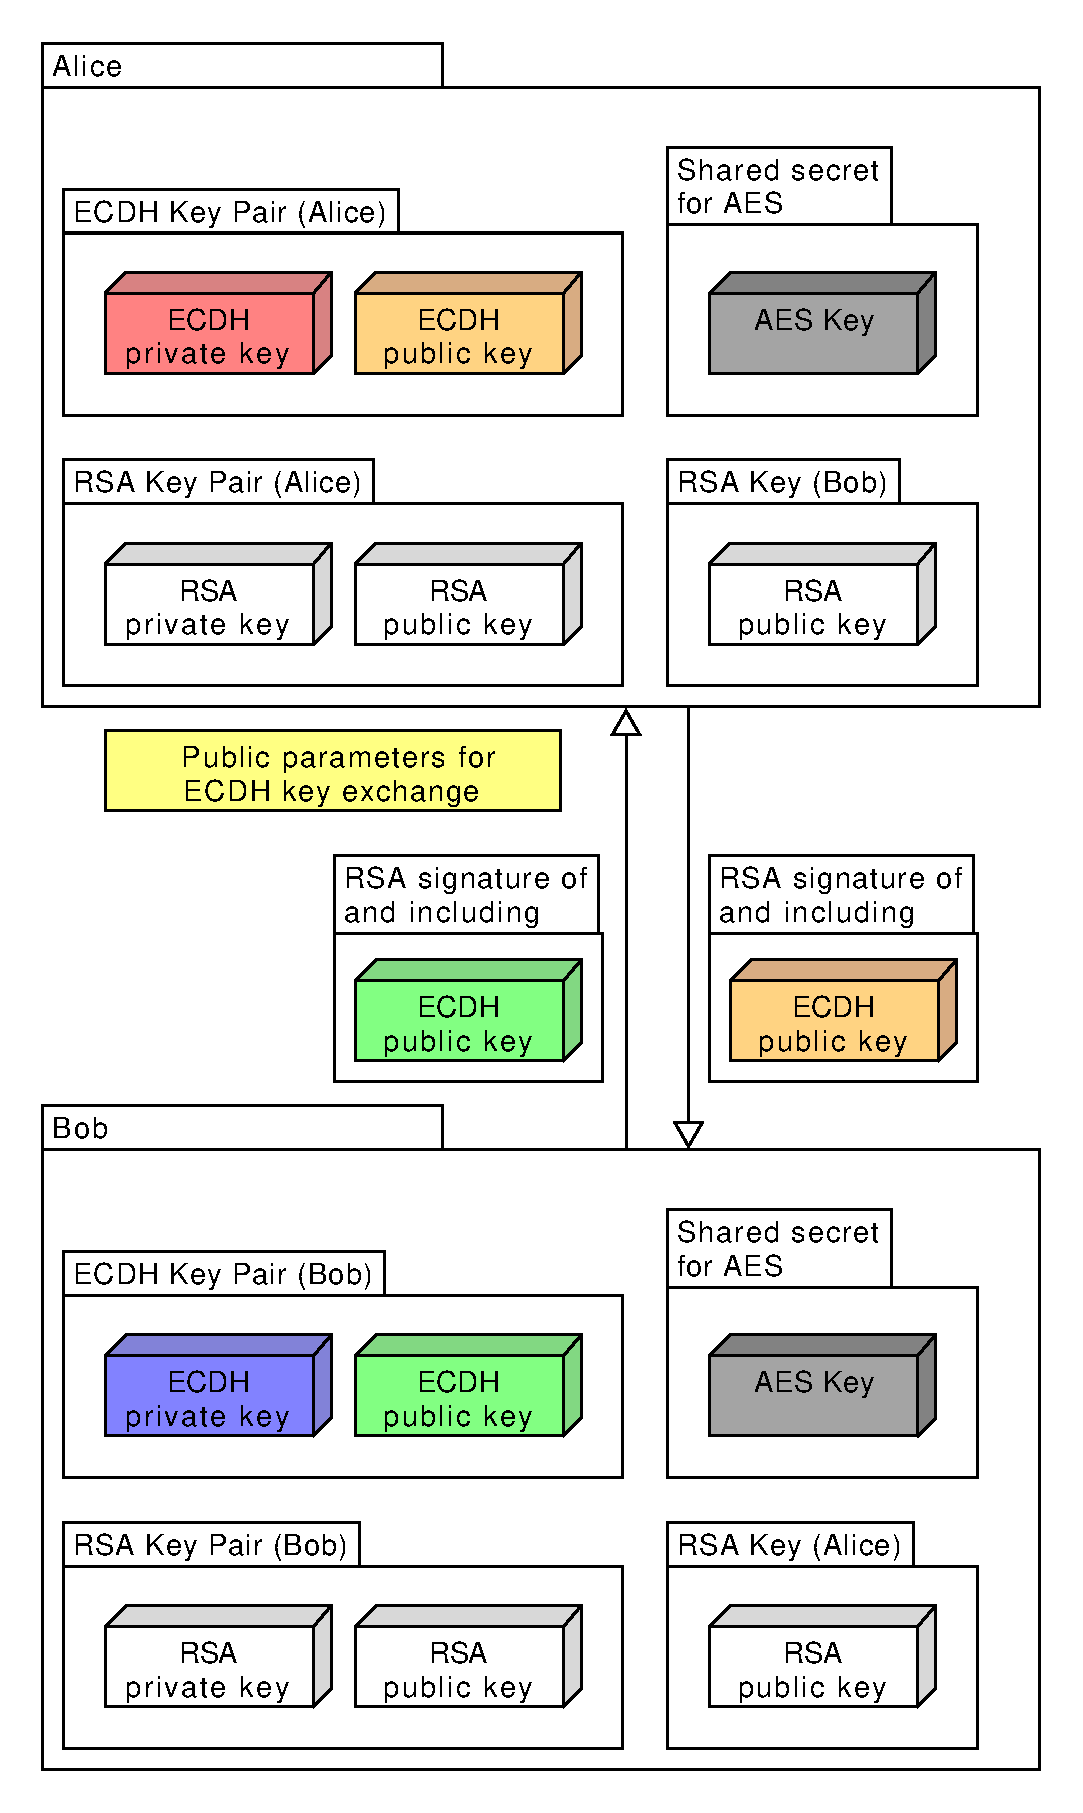
\includegraphics[width=1.0\textwidth]{./graphics/encryption}
    \caption{Trale Network Architecture}
    \label{fig:figure45}
\end{figure}




\begin{figure}[H]
    \centering
    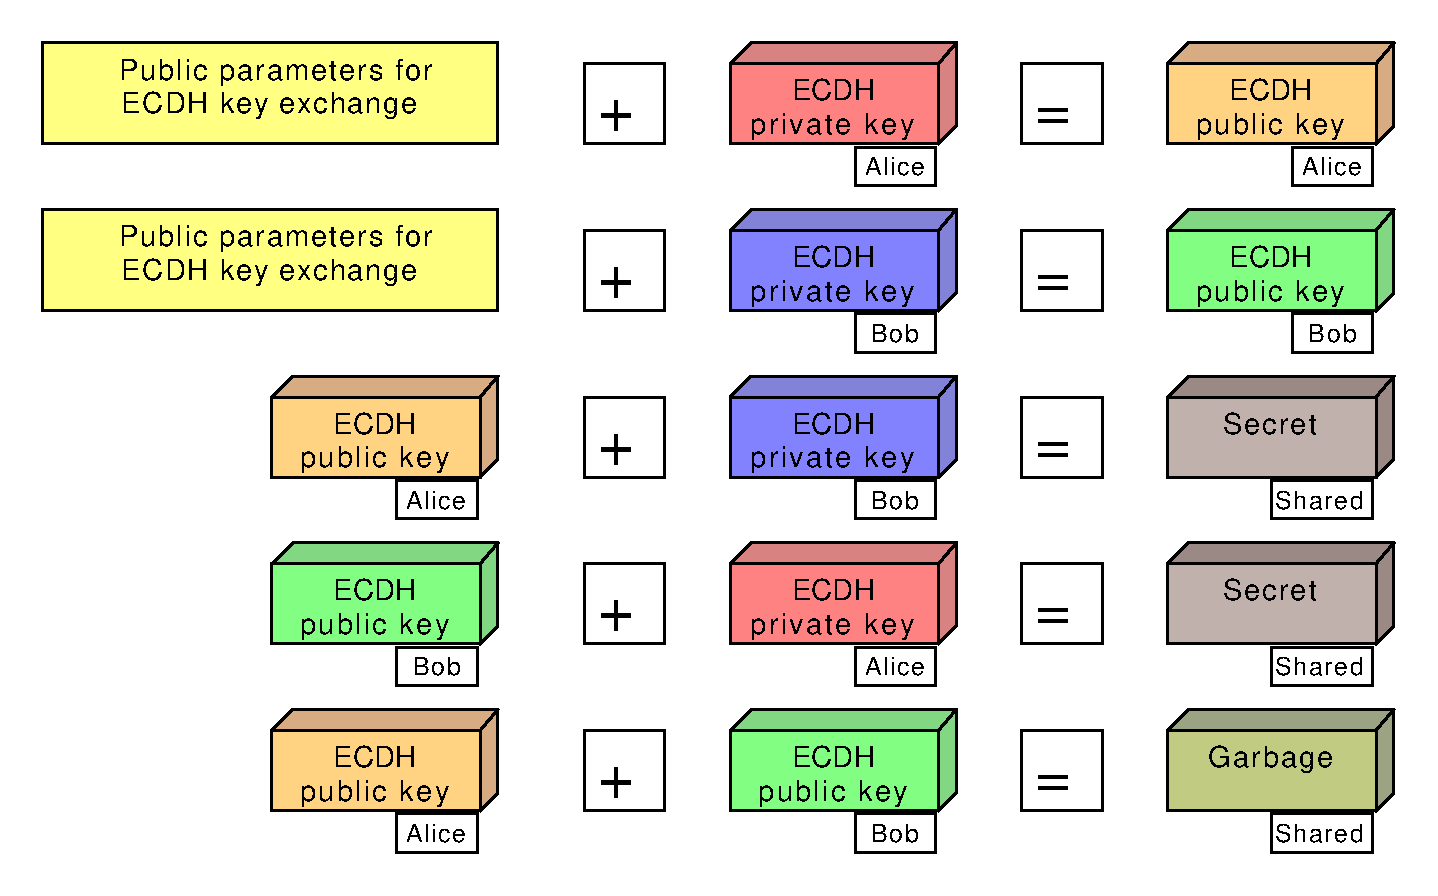
\includegraphics[width=1.0\textwidth]{./graphics/encryptionPattern.pdf}
    \caption{Trale Network Architecture}
    \label{fig:figure46}
\end{figure}

% TODO @joernneumeyer LG3:
% Define a research topic relevant to the project, do the research, report on it and care for adequate
% application of the results in the project

% Encryption algorithms --> AES, RSA, ECDH --> which one is best for Trale? Why? Draw decision process...
% related to LG 1: [...] criteria-based decision-making [...]
